\subsection{Projektumfeld}
\label{sec:Projektumfeld}

Neben der Projektgruppe \acs{VCL} sind noch viele weitere Personen an dem
Projekt beteiligt. Alle diese Personen stellen Stakeholder in diesem dar.
Stakeholder sind hierbei alle Personen, die ein berechtigtes Interesse sowohl
an dem Verlauf als auch an dem Ergebnis des Projektes haben. Alle
beteiligten Stakeholder lassen sich den Rollen "`Entwickler"', "`Auftraggeber"',
"`Betreuer"', "`Berater"' und "`Anwender"' zuordnen. Im Folgenden sollen die
Besonderheiten der einzelnen Rollen und die Personen, die diese Rollen besetzen,
genauer beschrieben werden, um einen besseren Einblick in das Projektumfeld zu
vermitteln.

Die Projektgruppe selbst übernimmt die Rolle der Entwickler im Projekt. Sie ist
somit für die Umsetzung der Projektidee und Realisierung der Projektziele
verantwortlich. Innerhalb der Projektgruppe wurde Raphael Otten als
Projektleiter ausgewählt. Er übernimmt hiermit im Projekt die Planung und
Steuerung und dient weiterhin als Schnittstelle zwischen Projektbetreuer und
Entwicklerteam. Weiterhin muss beachtet werden, dass das Projekt über die Dauer
von zwei Semestern realisiert werden muss. Die vier Projektmitglieder befinden
sich daher zeitweise in der Praxisphase und können somit während der regulären
Arbeitszeit nicht an dem Projekt arbeiten. Diese Tatsache stellt besondere
Anforderungen an die Organisation der Projektgruppe.

Da die Fakultät Management, Kultur und Technik am Standort Lingen ansässig ist,
stellt die Leitung dieser Fakultät die Rolle des Auftraggebers im Projekt dar.
Die Fakultätsleitung besteht hierbei aus dem Dekan der Fakultät, Prof. Dr. Frank
Blümel, und den Leitern der vier Institute der Fakultät. Diese sind:

\begin{itemize}
  \item Prof. Dr. Michael Ryba (Institut Management und Technik)
  \item Prof. Dr.-Ing. Wolfgang Arens-Fischer (Institut für Duale Studiengänge)
  \item Prof. Dr. Dagmar Schütte (Institut für Kommunikationsmanagement)
  \item Prof. Dr. Bernd Ruping (Institut für Theaterpädagogik)
\end{itemize}

Alle Mitglieder des Gremiums sind innerhalb ihres Instituts stark eingebunden.
Aus diesem Grund muss für ein gemeinsames Treffen zwecks Projektabsprache mit
allen Mitgliedern eine sehr lange Vorlaufzeit eingeplant werden. Bei einem
solchen Treffen mit der Fakultätsleitung sollten der Projektnutzen und das
Projektziel im Vordergrund stehen, da dieses Gremium über die Realisierung und
spätere Einführung des Projektes entscheidet.

Die Rolle der Betreuer im Projekt wird von den Projektpaten Herrn Stephan
Feldker und Herrn Prof. Dr.-Ing. Ralf Westerbusch übernommen. Diese sollen der
Projektgruppe bei Fragen zur Seite stehen und durch den Prozess der
Projektumsetzung begleiten. Hierfür müssen die Betreuer in das Projekt mit
eingebunden und über den aktuellen Stand des Projektes informiert werden. Die
Betreuer stellen weiterhin die Schnittstelle der Kommunikation zwischen der
Projektgruppe und der Fakultätsleitung dar.

Bei der Umsetzung des Projektes strebt die Projektgruppe eine visuelle
Darstellung des Campus Lingen an. Es ist somit sehr Wahrscheinlich, dass die
Umsetzung die Veröffentlichung von Fotos beinhaltet, auf denen die
Räumlichkeiten und Studenten des Campus dargestellt sind. Um die Projektgruppe
bei datenschutzrechtlichen Fragen zu unterstützen wurde von Herrn Feldker der
Kontakt zum Datenschutzbeauftragten der Hochschule Osnabrück, Prof. Dr. Alfred
Scheerhorn, hergestellt. Dieser ist somit als Berater an dem Projekt beteiligt
und gehört zum Kreis der Stakeholder.

Auch die Anwender des zu realisierenden Systems gehören zu den Stakeholdern im
Projekt. Das Projekt richtet sich hierbei, wie bereits in dem
\verweis{Projektidee} erwähnt, an Studieninteressierte und potenzielle
Studenten. Die Interessen dieser Zielgruppe müssen bei der Umsetzung des
Projektes berücksichtigt werden.

Ein Überblick über alle Stakeholder ist in \abbildung{Stakeholder} dargestellt.

\begin{figure}[htb] 
\centering
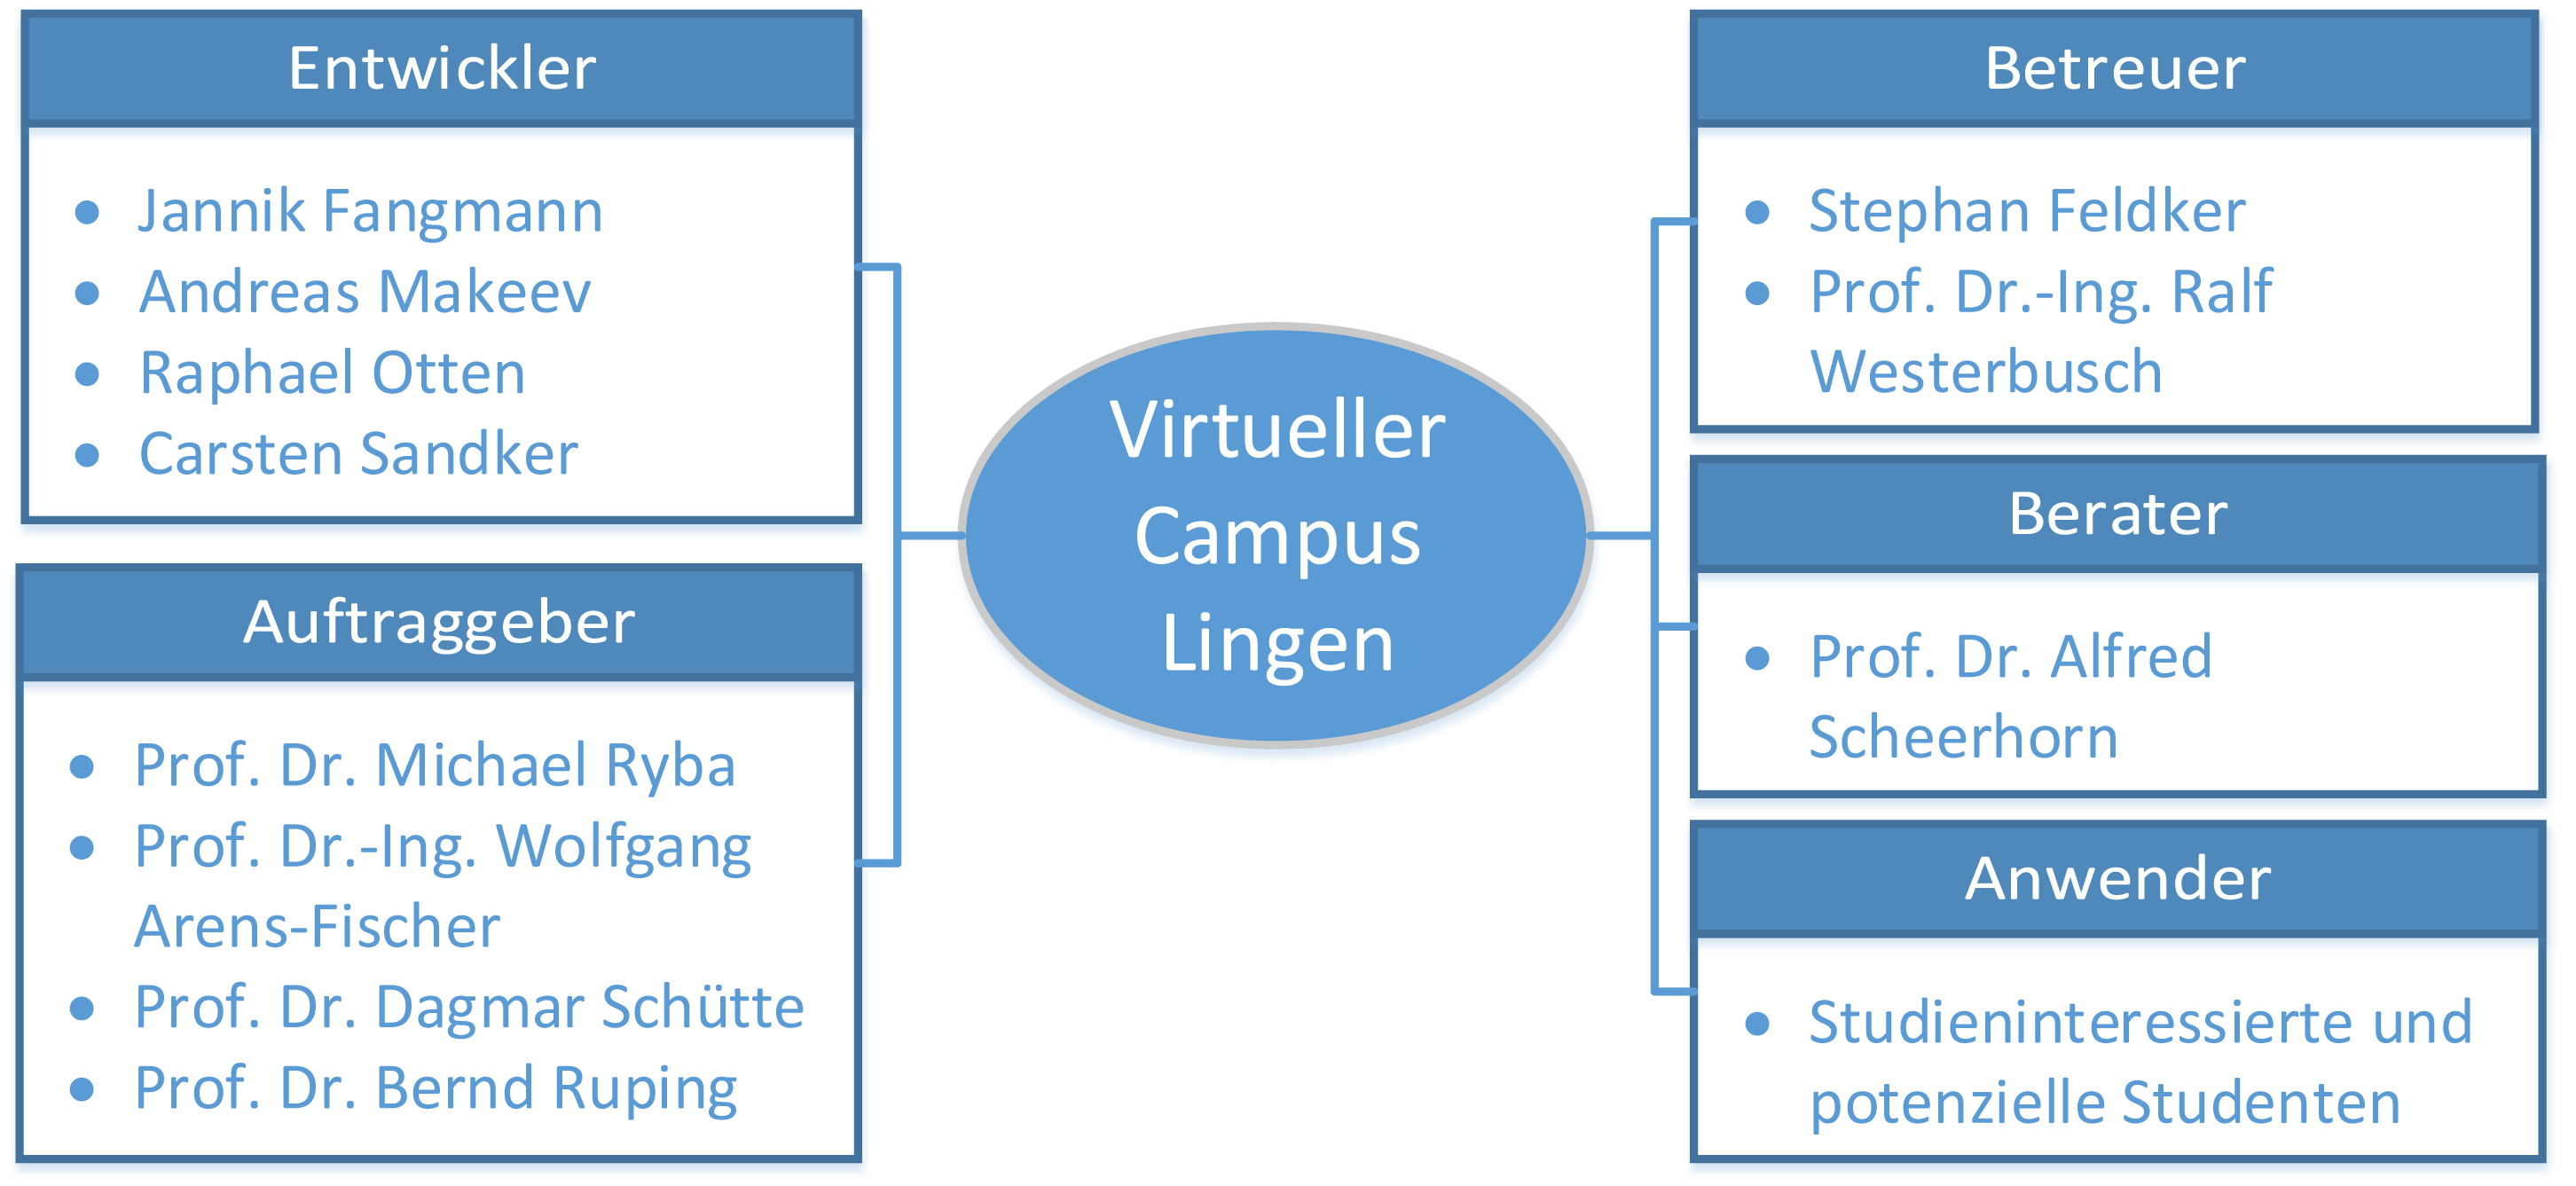
\includegraphics[width=0.8\textwidth]{Stakeholder.png}
\caption[Stakeholder im Projekt \acs{VCL}]{Stakeholder im Projekt \acs{VCL}\protect\footnotemark}
\label{fig:Stakeholder}
\end{figure}
\footnotetext{Eigene Darstellung}
